\documentclass{standalone}
\usepackage{graphicx}
\usepackage{float}
\usepackage[caption=false,font=normalsize,labelfont=small,textfont=sf]{subfig}
\usepackage{amsmath,amssymb}
\begin{document}

\begin{figure*}[ht]
    \centering
    \subfloat[]{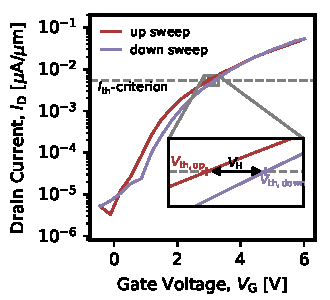
\includegraphics[]{figures/hysteresis_IdVg_example.pdf}\label{fig:example_hyst_IdVg}}
    \hfill
    \subfloat[]{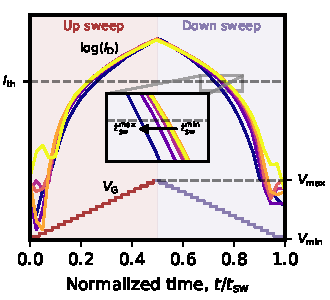
\includegraphics[]{figures/hysteresis_time_example.pdf}\label{fig:hysteresis_vs_time}}
    \hfill
    \subfloat[]{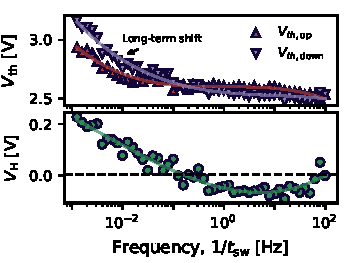
\includegraphics[]{figures/hysteresis_Vth_DeltaVth_vs_freq.pdf}\label{fig:hysteresis_vs_freq}} \\[-1.2em]
    \subfloat[]{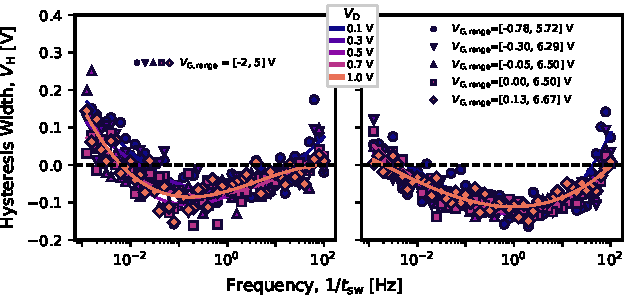
\includegraphics[]{figures/hysteresis_DeltaVth_vs_freq_differentVd.pdf}\label{fig:hyst_differentVd}}
    \hfill
    \subfloat[]{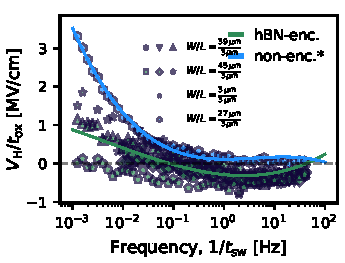
\includegraphics[]{figures/hysteresis_DeltaVth_vs_freq_comparison.pdf}\label{fig:hyst_comparison}} 
    \caption{(a) \textbf{Typical hysteresis curve}: the hysteresis width, $V_\mathsf{H}$, is defined as the difference between the threshold voltages extracted during the up and down sweeps, i.e., $V_{H} = V_\mathsf{th,up} - V_\mathsf{th,down}$. (b) \textbf{Hysteresis dependence on the gate voltage sweep rate}: $\log(I_{D})$ and $V_\mathsf{G}$ are shown as a function of the normalized sweep time, $t/t_\mathsf{sw}$, for different sweep rates, $r_\mathsf{sw}$. (c) \textbf{Hysteresis-$r_\mathsf{sw}$ curves}: Threshold voltages, $V_\mathsf{th,up}$ and $V_\mathsf{th,down}$, and hysteresis width, $V_\mathsf{H}$, are shown as a function of the sweep rate, $r_\mathsf{sw}$.}
    \label{fig:hysteresis}
\end{figure*}

\end{document}